\documentclass[thesis.tex]{subfiles}

\begin{document}

\subsection{Simplicial complexes and Ranicki duality}

In this section, the theory developed in the previous one is specialized in two ways. Only posets associated with simplicial complexes are considered and the sheaves and cosheaves studied have values either in the category of abelian groups $\Ab$ or its full subcategory $\Ab_{\f}$ of finitely generated abelian groups.

The notion of tensor product of functors is used to define the tensor product of a complex of sheaves and a complex of cosheaves. In conjunction with linear duality and a couple of special complexes, this tensor product is used to define the Ranicki duality functors, whose geometric content is made apparent by the pair subdivision sheaf and cosheaf.

The section closes with the construction, using the pair subdivision sheaf, of the visible symmetric complex of a regular pseudomanifold.

\begin{definition}\label{Posets <-- SC}
Consider the category $\SC$ of ordered simplicial complexes as presented in Definition \ref{ordered simplicial complexes}. Define a functor $$\SC\to\Poset$$ sending an ordered simplicial complex $X=(V,S)$ to the poset $(S,\leq)$ with $\sigma\leq\tau$ if an only if $\sigma\subset\tau$, i.e. if $\sigma$ is a face of $\tau$.

For any $X\in\SC$, define the categories of \textbf{sheaves and cosheaves on $X$}, denoted $\Sh(X)$ and $\coSh(X)$, to be the corresponding sheaves and cosheaves categories on its associated poset.

The \textbf{barycentric subdivision functor} $\SC\to\SC$ is defined as the composition of the functor defined above and the functor $\Poset\to\SC$ sending a poset $(P,\leq)$ to the simplicial complex with $P$ as set of vertices and simplices given by strictly ascending sets $[\sigma_0<\dotsb<\sigma_n]$ of elements in $P$.
\end{definition}

\begin{definition}(Open star and closure)
Let $X$ be an ordered simplicial complex and $\sigma$ a simplex in $X$. The \textbf{open star} of $\sigma$, denote by $\st\sigma$, is defined as the subset of $X$ formed by all simplices containing $\sigma$. The \textbf{closure} of $\sigma$, denote by $\cl\sigma$, is defined as the subcomplex of $X$ formed by all simplices contained in $\sigma$. Notice that if $\sigma\leq\tau$ then $\st\sigma\supset\st\tau$ and $\cl\sigma\subset\cl\tau$.
\end{definition}

\begin{definition}\label{sheaf of cochains and cosheaf of chains}
The complex of sheaves $\cochains$ with values in $\Ab$ is defined to assign to each simplex the chain complex of cochains on its open star, i.e. $$\cochains[\sigma]=\big(\!\cochains(\st\sigma),\delta\big),$$
and to have induced morphisms given by inclusions.

The complex of cosheaves $\chains$ with values in $\Ab$ is defined to assign to each simplex the chain complex of cochains on its closure, i.e. $$\chains[\sigma]=\big(\!\chains(\cl\sigma),\partial\big),$$
and to have induced morphisms given by inclusions.
\end{definition}

The following definition is presented in level of generality suitable for the purposes of this work. For a more general discussion see for example \cite{Rie14}.
\begin{definition}(Tensor products of functors) \label{tensor product of functors}
Consider a pair of functors $F:\C^{\op}\to\Ab$ and $G:\C\to\Ab$. The \textbf{tensor product of $F$ and $G$ over $\C$} is defined by
$$F\stackrel[\C]{}{\tensor}G=\coeq\Big(\!\bigoplus_{f:\,c_1\to c_2}\!F(c_2)\tensor G(c_1)\,\rightrightarrows\,\bigoplus_{c}\,F(c)\tensor G(c)\Big),$$
and the \textbf{tensor product of $G$ and $F$ over $\C$} is defined by
$$G\stackrel[\C]{}{\tensor}F=\coeq\Big(\!\bigoplus_{f:\,c_1\to c_2}\!G(c_1)\tensor F(c_2)\,\rightrightarrows\,\bigoplus_{c}\,F(c)\tensor G(c)\Big).$$
\end{definition}

\begin{example} Let $R$ be a ring thought of as a category enriched over $\Ab$ with a single object. A right $R$-module corresponds to an $\Ab$-enriched functor $A:R^{\op}\to\Ab$, while a left $R$-module corresponds to an $\Ab$-enriched functor $B:R\to\Ab$. The functor tensor product $A\tensor_R B$ agrees with the usual tensor product of a left and a right $R$-module.
\end{example}

\begin{definition}
Given $\D\in\Sh(X)$ and $\E\in\coSh(X)$ define the sheaf $\E\stackrel[\,\st]{}{\stensor}\D$ by $$(\E\stackrel[\,\st]{}{\stensor}\D)[\sigma]=\E|_{\st\sigma}\stackrel[\,\st\sigma]{}{\tensor}\D|_{\st\sigma}=\bigoplus_{\sigma\leq\tau}\E[\tau]\tensor\D[\tau]\big/\sim$$
with $\big(\D[\iota](e)\tensor d\big)\sim\big(e\tensor \E[\iota](d)\big)$ for any $\iota:\sigma\to\tau$, and morphisms being induced by inclusions.

Analogously, define the cosheaf $\E\stackrel[\cl]{}{\stensor}\D$
$$(\E\stackrel[\,\cl]{}{\stensor}\D)[\sigma]=\E|_{\cl\sigma}\stackrel[\,\cl\sigma]{}{\tensor}\D|_{\cl\sigma}=\bigoplus_{\rho\leq\sigma}\E[\rho]\tensor\D[\rho]/\sim$$
with $\big(\E[\iota](e)\tensor d\big)\sim\big(e\tensor \D[\iota](d)\big)$ for any $\iota:\rho\to\sigma$, and morphisms being induced by inclusions.

These assignments are functorial in both variables. The notation $\stensor_{\st}$ and $\stensor_{\cl}$ will also be used for the extension of these bifunctors to complexes.
\end{definition}

\begin{remark}\label{Z x E = E and D x Z = D}
Fix an ordered simplicial complex $X$. Let $\underline{\Z}$ be the constant cosheaf on $X$ with value $\Z$. For any sheaf $\D$ the collection of maps
$$\big(\underline{\Z}\stackrel[\,\st]{}{\stensor}\D\big)[\sigma]=\Big(\bigoplus_{\sigma\leq\tau}\Z_\tau\tensor\D[\tau] /\sim\Big)\,\to\,\D[\sigma]$$ sending $1_\tau\tensor d$ to $\D[\iota](d)$ with $\iota:\sigma\to\tau$ defines an isomorphism of sheaves.

Analogously, let $\overline{\Z}$ be the constant sheaf. For any cosheaf $\E$ the collection of maps
$$\big(\E\stackrel[\,\cl]{}{\stensor}\overline{\Z}\big)[\sigma]=\Big(\bigoplus_{\rho\leq\sigma}\E[\rho]\tensor\Z_\rho /\sim\Big)\,\to\,\E[\sigma]$$ sending $e\tensor1_\rho$ to $\E[\iota](e)$ with $\iota:\rho\to\sigma$ defines an isomorphism of cosheaves.
\end{remark}

\begin{notation}
Let $(-)^{\vee}:\Sh(X,\Ab)\to\coSh(X,\Ab)$ be the functor induced from linear duality. Explicitly, for any $\D\in\Sh(X,\Ab)$ one has
$$\D^{\vee}[\sigma]=(\D[\sigma])^{\vee}\text{ and }\D^{\vee}[\iota]=(\D[\iota])^{\vee}\text{ for all } \iota:\sigma\to\tau.$$
Since the context will be clear enough to avoid confusions, the analogous functor $\coSh(X,\Ab)\to\Sh(X,\Ab)$ will be denoted by the same symbol $(-)^{\vee}$.

The same notation $(-)^\vee$ will be used for the extension of these functors to complexes.
\end{notation}

\begin{definition} (Ranicki duality functors)\label{Ranicki duality functors}
Let $X$ be an ordered simplicial complex. Abusing notation, define respectively the \textbf{Ranicki duality functors} $\T:\Sh(X,\Ab)_\bullet\to\Sh(X,\Ab)_\bullet$ and $\T:\coSh(X,\Ab)_\bullet\to\coSh(X,\Ab)_\bullet$ as the following compositions $$\T(-)=(-)^{\vee}\stackrel[\,\st]{}{\stensor}\cochains\text{\ \ and\ \ } \T(-)=\chains\stackrel[\,\cl]{}{\stensor}(-)^{\vee}.$$
\end{definition}

\begin{example}
Notice that $\overline{\Z}^{\vee}\cong\underline{\Z}$ and $\underline{\Z}^{\vee}\cong\overline{\Z}$, so by Remark \ref{Z x E = E and D x Z = D} one has $\T\overline{\Z}\cong\cochains$ and $\T\underline{\Z}\cong\chains$.
\end{example}

\begin{example}
Let $X$ be the interval an represent $\cochains$ and $\chains$ by

\begin{minipage}[c]{6cm}
$$\ \ \cochains: \ \ \xymatrix@C=10pt @R=10pt{
\alpha \ar[d]_{-1} & & & &\gamma \ar[d]^{+1}\\
\beta  & & \ar@{_{(}->}[ll]\, \beta \,\ar@{^{(}->}[rr] & &\beta \\
\bullet & \ar@{-}[rr]& & & \bullet }$$
\end{minipage}
\begin{minipage}[c]{6cm}
$$\chains: \ \ \ \ \xymatrix @C=11pt @R=10pt{
  & & \ar[dl]_{-1} b \ar[dr]^{+1} & & \\
a \,\ar@{^{(}->}[r] &a & &c &\ar@{_{(}->}[l]\, c  \\
\bullet & \ar@{-}[rr]& & & \bullet . }$$
\end{minipage}\vspace*{20pt}\\
Their linear duals are represented by

\begin{minipage}[c]{6cm}
$$(\cochains)^{\vee}:\ \xymatrix@C=12pt @R=11pt{
b  \ar@{->>}[rr]& & b & & \ar@{->>}[ll] b \\
a \ar@{<-}[u]^{-1} & & & & c \ar@{<-}[u]_{+1}\\
\bullet & \ar@{-}[rr]& & & \bullet }$$
\end{minipage}
\begin{minipage}[c]{6cm}
$$(\chains)^{\vee}: \ \, \xymatrix @C=9pt @R=10pt{
\alpha & \ar@{->>}[l] \alpha & & \gamma \ar@{->>}[r] & \gamma  \\
  & & \ar@{<-}[ul]^{-1} \beta \ar@{<-}[ur]_{+1} & & \\
\bullet & \ar@{-}[rr]& & & \bullet .}$$
\end{minipage}\vspace*{20pt}\\
The Ranicki dual of $\cochains$ defined as $(\cochains)^{\vee}\stackrel[\,\st]{}{\stensor}\cochains$ is represented by

$$\T\cochains:\ \xymatrix@C=12pt @R=11pt{
 &\ar[dl]_{-1}b\alpha\ar[dr]^{+1}& & & & & &\ar[dl]_{-1}b\gamma\ar[dr]^{+1}& \\
a\alpha& &b\beta& &\ar@{_{(}->}[ll]\, b\beta \,\ar@{^{(}->}[rr]& &b\beta& &c\gamma\\
 &\bullet& &\ar@{-}[rr] & & & &\bullet.&}$$\\
The Ranicki dual of $\chains$ defined as $\chains\stackrel[\,\cl]{}{\stensor}(\chains)^{\vee}$ is represented by

$$\T\chains:\ \xymatrix@C=12pt @R=11pt{
& & &\ar[dl]_{-1}b\alpha\ar[dr]^{+1}& &\ar[dl]_{-1}b\gamma\ar[dr]^{+1}& & & \\
a\alpha\,\ar@{^{(}->}[rr]& &a\alpha& &b\beta& &c\gamma& &\ar@{_{(}->}[ll]\,c\gamma\\
\bullet& \ar@{-}[rrrrrr]& & & & & & &\bullet.}$$

Observe that in this example the collection of evaluation maps $$(\cochains[\sigma])^{\vee}\tensor\cochains[\sigma]\to\Z$$ induces a morphism of complexes of sheaves
$$\varepsilon:\T\cochains=\T^2\overline{\Z}\to\overline{\Z}$$ with $\varepsilon[\sigma]$ a homology isomorphism for every simplex $\sigma$.

Similarly defined, the morphism $$\varepsilon:\T\chains=\T^2\underline{\Z}\to\underline{\Z}$$ is a homology isomorphism over each simplex.
\end{example}

\begin{definition}(Pair subdivision) For any finite ordered simplicial complex define its \textbf{pair subdivision sheaf} $\Ps$ as the Ranicki dual of the complex of sheaves $\cochains$. Explicitly, one has chain isomorphisms
$$\Ps[\rho]\cong\big(\bigoplus_{\rho\leq\sigma,\tau}\tau\tensor\sigma^*\big)/\big(\bigoplus_{\sigma\nleq\tau}\tau\tensor\sigma^*\big)$$
with maps $\Ps[\rho\to\rho']:\Ps[\rho']\to\Ps[\rho]$ given by inclusions.

Define the \textbf{pair subdivision cosheaf} similarly by $$\Pcs=\T\chains=\chains\stackrel[\,\cl]{}{\stensor}(\chains)^\vee.$$
\end{definition}

\begin{remark}\label{pair subdivision related to dual cones}
The pair subdivision sheaf has a geometric interpretation justifying its name. Let $X$ be an ordered simplicial complex and $X'$ its barycentric subdivision as defined in \ref{Posets <-- SC}. For any $\rho\in X$ define the \textbf{close dual cone} of $\rho$, denoted $\dc(\rho)$, as the subcomplex of $X'$ containing all simplices of the form $[\rho_1<\rho_2<\dotsb]$ with $\rho\leq\rho_1$. The chain complex $\Ps[\rho]$ is chain isomorphic to the chain complex of a regular CW complex obtained by gluing along common faces certain simplices of $\dc(\rho)$. Two simplices in the closed dual cone are amalgamated along their common face if they have the same dimension and are represented by ascending subsets with the same initial and terminal simplices. For example, in the case of the (geometric realization of the) $2$-dimensional simplex the amalgamation map looks as follows:\vspace*{0pt}

\begin{minipage}{6cm}
\begin{center}\hspace*{3cm}
    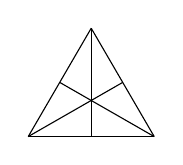
\begin{tikzpicture}[scale=1.6, every node/.style={scale=2.6}]
    \draw[black] (0,0) -- (0.5,0);
    \draw[black] (0.5,0) -- (1,0);
    \draw[black] (0,0) -- (0.5,0.86);
    \draw[black] (1,0) -- (0.5,0.86);

    \draw[black] (0.5,0) -- (0.5,0.86);
    \draw[black] (1,0) -- (0.25,0.43);
    \draw[black] (0,0) -- (0.75,0.43);
    \end{tikzpicture}
\end{center}
\end{minipage}
\begin{minipage}{1cm}
\vspace*{-.6cm}$$\longrightarrow$$
\end{minipage}
\begin{minipage}{6cm}
    \begin{center}
    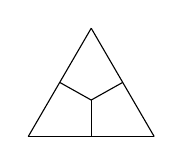
\begin{tikzpicture}[scale=1.6, every node/.style={scale=2.6}]
    \draw[black] (0,0) -- (0.5,0);
    \draw[black] (0.5,0) -- (1,0);
    \draw[black] (0,0) -- (0.5,0.86);
    \draw[black] (1,0) -- (0.5,0.86);

    \draw[black] (0.5,0.29) -- (0.5,0);
    \draw[black] (0.5,0.29) -- (0.25,0.43);
    \draw[black] (0.5,0.29) -- (0.75,0.43);
    \end{tikzpicture}\hspace*{3.2cm}
\end{center}
\end{minipage}\vspace*{10pt}

The subdivision map, which is the inverse of the amalgamation one defined above, induces a chain homotopy equivalence from $\Ps[\rho]$ into the chains on the dual cone of $\rho$ which are denoted $\DC[\rho]$. Notice that $\DC$ defines a complex of projective sheaves and, since $\Ps$ is also projective, the complexes $\DC$ and $\Ps$ are chain homotopy equivalent be Lemma \ref{Projective resolutions and weak => strong for projectives}. In particular, $\Ps[\rho]$ is contractible for all $\rho\in X$. See \cite{Rou10} for more on the pair subdivision complex.
\end{remark}

The Ranicki duality functors $\T$ are not in general involutions, not even up to homotopy. In order to have an involution-like property one needs to impose some finiteness conditions. This is accomplished by restricting $\T$ to $\Sh_{\c}(X,\Ab_{\f})_\bullet$ and $\coSh_{\c}(X,\Ab_{\f})_\bullet$, i.e. the categories of complexes of compactly supported sheaves, respectively cosheaves, with values in the category of finitely generated abelian groups.
\begin{lemma}\label{T^2 = id}
There exist natural transformations
$$\varepsilon:\T^2\to\id_{\Sh_{\c}(X,\Ab_{\f})}\text{\ \ \  and \ \ \ }\varepsilon:\T^2\to\id_{\coSh_{\c}(X,\Ab_{\f})}$$
defined below, such that if $\P_\bullet$ stands for a complex of projective sheaves or cosheaves then
\begin{enumerate}
\item The following pairs of complexes are chain isomorphic
$$\T^2\P_\bullet\cong \P_\bullet\stackrel[\,\st]{}{\stensor}\Ps \text{\ \ \  and \ \ \ } \T^2\P_\bullet\cong\P_\bullet\stackrel[\,\cl]{}{\stensor}\Pcs$$
\item The morphism $\varepsilon_{\P_\bullet}:(\T^2\P_\bullet)\to\P_\bullet$ is a chain homotopy equivalence.
\item The following diagram commutes
$$\xymatrix{\T\P_\bullet \ar[r]^-{\T(\varepsilon_{\P_\bullet})} \ar[rd]_-{\id} & \T^3\P_\bullet \ar[d]^-{\varepsilon_{\T\P_\bullet}} \\ &\T\P_\bullet.}$$
\end{enumerate}
\begin{proof}
Only the proof for sheaves will be presented since small variations adapt it for cosheaves. For any simplex $\sigma\in X$ denote its $i$-th face by $\partial_i\sigma$ and by $\delta^i\sigma$ any simplex such that $\partial_i\delta^i\sigma=\sigma$, notice that if $\delta^i\sigma$ exists then it is unique.

For any complex of sheaf $\D_\bullet$ one has  $\displaystyle{\T\D_\bullet[\rho]=\big(\bigoplus_{\rho\leq\sigma}\D_\bullet^\vee[\sigma]\tensor\cochains[\sigma]/\sim\big)}$ which equals $\displaystyle{\big(\bigoplus_{\rho\leq\sigma\leq\sigma'}\D_\bullet^\vee[\sigma]\tensor\cochains[\sigma\leq\sigma']\sigma'^*/\sim\big)}$. Using that $$d_\sigma^*\tensor\cochains[\sigma\leq\sigma'](\sigma'^\ast)\sim\D_\bullet^\vee[\sigma\leq\sigma'](d_\sigma^*)\tensor \sigma'^\ast$$ one sees that as graded abelian groups $$\T\D_\bullet[\rho]\cong\bigoplus_{\rho\leq\sigma}\D_\bullet^\vee[\sigma]\tensor\sigma^*.$$ This isomorphism can be improved to a chain isomorphism by setting
$$\partial(d_\sigma\tensor\sigma^*)=\partial d_\sigma\tensor\sigma^*+(-1)^{|d_\sigma|}\sum_{\delta^i\sigma}(-1)^i\D_\bullet^\vee[\sigma\leq\delta^i\sigma](d_\sigma)\tensor(\delta^i\sigma)^*.$$

Applying the previous observation twice and using the finite dimensionality of the abelian groups involved one has that as graded abelian groups
$$\T^2\D_\bullet[\rho]\cong\bigoplus_{\rho\leq\sigma\leq\tau}\D_\bullet[\tau]\tensor\tau\tensor\sigma^*.$$
To describe the boundary making this into a chain isomorphism observe that $(\T\D_\bullet)^\vee[\sigma\leq\sigma']:\bigoplus_{\sigma\leq\tau}\D_\bullet[\tau]\tensor\tau\to\bigoplus_{\sigma'\leq\tau}\D_\bullet[\tau]\tensor\tau$ is giving by projection. The boundary in $\displaystyle{\bigoplus_{\rho\leq\sigma\leq\tau}\D_\bullet[\tau]\tensor\tau\tensor\sigma^*}$ making it chain isomorphic to $\T^2\D_\bullet[\rho]$ is therefore
\begin{align*}
\partial(d_\tau\tensor\tau\tensor\sigma^*)=&\ \ \partial(d_\tau)\tensor\tau\tensor\sigma^*\\
&+ (-1)^{|d_\tau|}\sum_{\partial^i\tau}(-1)^i\D_\bullet[\partial_i\tau\leq\tau](d_\tau)\tensor\partial_i\tau\tensor\sigma^*\\
&+(-1)^{|d_\tau|+|\tau|}\sum_{\delta^i\sigma\leq\tau}(-1)^id_\tau\tensor\tau\tensor(\delta^i\sigma)^*.
\end{align*}
The above formula conceptually simplifies if $\D_\bullet$ is projective. In that case $\D[\partial_i\tau\leq\tau]$ is an inclusion map and the chain complex $\T^2[\rho]$ becomes chain isomorphic to $\D[\rho]\tensor\Ps[\rho]$.

For any $\D_\bullet$ define $\varepsilon_{\D_\bullet}[\rho]:\T^2\D_\bullet[\rho]\to\D_\bullet[\rho]$ by sending $d_\tau\tensor\tau\tensor\sigma^*$ to $\D_\bullet[\rho\leq\tau](d_\tau)\cdot\langle\tau,\sigma^*\rangle$. Using the formula for the boundary it can be shown this defines a morphism of complexes of sheaves. In case $\D_\bullet$ is projective then $\varepsilon_{\D_\bullet}[\rho]:\D_\bullet[\rho]\tensor\Ps[\rho]\to\D_\bullet[\rho]$ is the identity in the first factor and contracts the second. It is therefore a homology isomorphism and by Lemma \ref{Projective resolutions and weak => strong for projectives} $\varepsilon_{\D_\bullet}$ is a chain homotopy equivalence.

The proof of the third part becomes a straightforward computation. Let $\P_\bullet$ be projective and consider any $\rho\in X$ and $(d_\sigma\tensor\sigma^*)\in\T\P_\bullet[\rho]$, then
$$\xymatrix@C=-3pc{\ \ \ \ \ (d^*_\sigma\tensor\sigma^*) \ar@{|->}[rr]^-{\T(\varepsilon_{\P_\bullet})[\rho]} \ar@{|->}[rd]^-{\id} & & d_\sigma^*\tensor\big(\sum_{\sigma\leq\tau}\tau^*\tensor\tau\big)\tensor\sigma^* \ar@{|->}[dl]_-{\varepsilon_{\T\P_\bullet}} \\
&\ \ \ \ \ \ \  d_\sigma^*\tensor\big(\sum_{\sigma\leq\tau}\tau^*\tensor\langle\tau,\sigma^*\rangle\big) & } $$
\end{proof}
\end{lemma}

\begin{remark}\label{S_2 action on Hom(T,)}
For any projective complex $\P_\bullet$ of compactly supported sheaves or cosheaves with values on $\Ab_{\f}$, the lemma above can be used to endow the chain complex $\Hom(\T\P_\bullet,\P_\bullet)$ with an action of $\Sigma_2$ defined to send $f$ to $(\varepsilon_{\P_\bullet}\circ\T f)$. This is an involution since
$$\varepsilon_{\P_\bullet}\circ\T(\varepsilon_{\P_\bullet}\circ\T f)=\varepsilon_{\P_\bullet}\circ\T^2 f\circ\T(\varepsilon_{\P_\bullet})=
f\circ\varepsilon_{\T\P_\bullet}\circ\T(\varepsilon_{\P_\bullet})=f.$$
\end{remark}

\begin{notation}\label{homotopy fix points}
Recall from Definition \ref{E infinity operad} that the arity $2$ part of the operad $\S$ carries a free action of $\Sigma_2$ and has the homology of a point. For any chain complex $C$ with an action of $\Sigma_2$, the chain complex of $\Sigma_2$-equivariant maps from $\S(2)$ to $C$ will be denoted $C^{\Sigma_2}$. Let $\varphi\in C^{\Sigma_2}$ and as in Example \ref{Delta_n on n-simplices (with signs)}, let $(\dotsc,2,1,2)$ be one of the degree $d$ generators of $\S(2)_\bullet$. The image of this generator via $\varphi$ will be denoted $\varphi_d$, and if $\varphi$ is a cycle then one has
$$\partial \varphi_{d+1}=(1-(-1)^{d}T)\varphi_{d}.$$
Cycles in $C^{\Sigma_2}$ can be therefore thought of as homotopy fix points of the $\Sigma_2$-action on $\C$, compare with Example \ref{fix points}.
\end{notation}

\begin{remark}\label{dual of pair subdivision related to relative dual cones}
Applying Lemma \ref{T^2 = id} to the pair subdivision sheaf one gets that $\varepsilon_{\Ps}:\T \Ps\cong \T^2\cochains\to \cochains$ is a chain homotopy equivalence.

Recall that by definition $\cochains[\sigma]$ is isomorphic to $\bigoplus_{\sigma\leq\tau}\tau^*$, the complex of cochains on the open star of $\sigma$. The concept of dual cone can be used to give another geometric interpretation for $\cochains$. Consider the amalgamation, described in Remark \ref{pair subdivision related to dual cones}, of the close dual cone of a simplex $\sigma$ into a subcomplex of the pair subdivision. The CW subcomplex corresponding to the open part of the dual cone of $\sigma$ is parametrized by simplices $\tau$ satisfying $\tau\geq\sigma$, with a simplex of dimension $k$ in the open star corresponds to a cell of dimension $k-|\sigma|$ in the amalgamated open dual cone. For example, \vspace*{6pt}

\begin{minipage}{4cm}
\begin{center}\hspace*{1.7cm}
    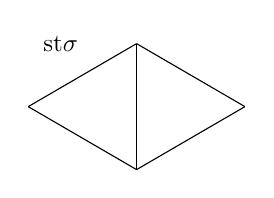
\begin{tikzpicture}[scale=1.6, every node/.style={scale=0.9}]
    \draw[black] (0,-.5) -- (0,.5)
    node[anchor=east] {$\mathrm{st}\sigma$\ \ \ \ \ \ \ };
    \draw[black] (0,.5) -- (-.86,0);
    \draw[black] (0,.5) -- (.86,0);
    \draw[black] (0,-.5) -- (-.86,0);
    \draw[black] (0,-.5) -- (.86,0);
    \end{tikzpicture}
\end{center}
\end{minipage}
\begin{minipage}{3cm}
\vspace*{-.6cm}$$\ \ \ \ \ \ \longrightarrow$$
\end{minipage}
\begin{minipage}{5cm}
\begin{center}
    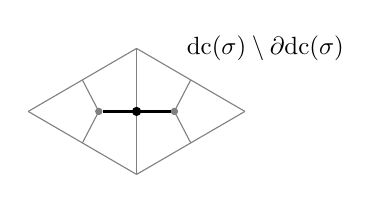
\begin{tikzpicture}[scale=1.6, every node/.style={scale=.9}]
    \draw[gray, thin] (0,-.5) -- (0,.5)
    node[anchor=west,black] {\ \ \ \ \ $\mathrm{dc}(\sigma)\setminus\partial\mathrm{dc}(\sigma)$};;
    \draw[gray, thin] (0,.5) -- (-.86,0);
    \draw[gray, thin] (0,.5) -- (.86,0);
    \draw[gray, thin] (0,-.5) -- (-.86,0);
    \draw[gray, thin] (0,-.5) -- (.86,0);

    \filldraw[black] (0,0) circle (.9pt);
    \filldraw[gray] (-.3,0) circle (.7pt);
    \filldraw[gray] (.3,0) circle (.7pt);

    \draw[black, thick] (0,0) -- (-.27,0);
    \draw[black, thick] (0,0) -- (.27,0);

    \draw[gray, thin] (-.3,0) -- (-.43,0.25);
    \draw[gray, thin] (-.3,0) -- (-.43,-0.25);
    \draw[gray, thin] (.3,0) -- (.43,0.25);
    \draw[gray, thin] (.3,0) -- (.43,-0.25);
    \end{tikzpicture}\hspace*{1.2cm}
\end{center}
\end{minipage}\vspace*{10pt}

This geometric correspondence induces a chain homotopy equivalence between $\cochains[\sigma]$ and $S^{-|\sigma|}\!\cochains(\dc\sigma,\partial\dc\sigma)$; the complex, suspended by $|\sigma|$, of relative cochains on the closed dual cone modulo its boundary.
\end{remark}

\begin{construction}\label{visible symmetric complex} The goal of this construction is to naturally obtain a degree $n$ cycle $\varphi$ in $\Hom_{\Sh}(\T\Ps,\Ps)^{\Sigma_2}$ when the base $X$ is a regular $n$-dimensional pseudomanifold. This will be done taking the following steps. First, a morphism
$$\DC[-]\to\Hom_{\Sh}(\Sigma^{|-|}\T\Ps[-],\Ps[-])^{\Sigma_2}$$
of complexes of sheaves will be constructed. Second, a collection of compatible homomorphism $\chains(X')\to\DC[\sigma]$ will be defined. third, the desired cycle will be obtained by evaluating the fundamental cycle of $\chains(X')$ in their composition.

Let $X$ be an ordered simplicial complex and $X'$ its barycentric subdivision. Let $\DC$, as in Remark \ref{pair subdivision related to dual cones}, be the projective complex of sheaves assigning to each $\sigma$ in $X$ the complex of simplicial chains in $\dc(\sigma)$, the dual cone of $\sigma$; and to each pair $\sigma\leq\tau$ the inclusion $\chains(\dc(\tau))\to\chains(\dc(\sigma))$.
Each of this complexes is in a functorial manner an $\S$-coalgebra and in particular an $\S(2)$-coalgebra, so by the hom-tensor adjunction the $\S(2)$-structures define a morphism of complexes of sheaves
\begin{equation*}
\DC[-]\to\Hom_{\Sigma_2}\big(\S(2),\DC[-]\tensor\DC[-]\big).
\end{equation*}
For every $\sigma\in X$ one has
$$\DC[\sigma]\tensor\DC[\sigma]\cong\Hom\!\Big(\!\!\cochains\big(\!\dc(\sigma)\,,X'\setminus\dc(\sigma)\big)\,,\DC[\sigma]\Big)$$
which is chain homotopy equivalent to
$$\Hom\!\Big(\!\!\cochains\big(\dc(\sigma)\,,\partial\dc(\sigma)\big)\,,\DC[\sigma]\Big).$$
This complex is by Remark \ref{dual of pair subdivision related to relative dual cones} chain homotopy equivalent to
$$\Hom\!\big(\Sigma^{|\sigma|}\T\Ps[\sigma]\,,\Ps[\sigma]\big),$$ so one gets a morphism of complexes of sheaves
\begin{equation}\label{eq: morphisms from cone sheaf to HOM one}
\DC[-]\to\Hom_{\Sigma_2}\big(\S(2),\Hom_{\Sh}\big(\Sigma^{|-|}\T\Ps[-],\Ps[-]\big)\big).
\end{equation}

For any chain in the simplicial chain complex of $X'$ one can construct an element in $\DC$ whose value in $\DC[\sigma]$ is computed by projecting the chain to the dual cone of the smallest vertex of $\sigma$, followed by taking its boundary and projecting it to the dual cone of the smallest edge of $\sigma$, and so on until reaching the projection to the dual cone of $\sigma$; in symbols if $\sigma=[v_0,\dotsc,v_n]$ one has
$$c\longmapsto\pi_{[v_0,\dotsc,v_n]}\circ\partial\circ\dotsb\circ\pi_{[v_0,v_1]}\circ\partial\circ\pi_{[v_0]}(c)$$
with $\pi_\sigma$ denoting the projection from the simplicial chain complex of $X'$ onto $\DC[\sigma]$. Notice that this construction decreases degree by $|\sigma|$.

Let $X$ be a simply connected regular pseudomanifold, i.e. an $n$-dimensional simplicial complex such that: each codimension $1$ face is the boundary of exactly two distinct $n$-dimensional simplices, the boundary of the star of each simplex of codimension at least $2$ is connected, and the sum of all $n$-dimensional simplices, denoted $[X]$, is a cycle. Passing to the barycentric subdivision, let $[X']$ denote the cycle corresponding to $[X]$. The image of $[X']$ in $\DC$ via the above construction is mapped by the morphism (\ref{eq: morphisms from cone sheaf to HOM one}) to an $n$-dimensional cycle $\varphi\in\Hom_{\Sh}(\T\Ps,\Ps)^{\Sigma_2}$. The pair $(\Ps,\varphi)$ will be referred to as the \textbf{visible symmetric complex} of $X$.
\end{construction}


\end{document}







